\tocless\subsection{Strict total order}

Given that our goal is to find a way to compare traces produced under the \tpl\ operational semantics, to the ones achieved from the \textsc{Atom} one, we need to establish a strict total order on the transactions that appear in a trace. The properties of such an order relation, enable us to effectively simulate a serial reduction, as we know that, from an abstract point of view, we can look at two parallel transactions as if one \textit{happens before} the other.

The serialization graph structure $(N, E) = \pred{SG}{\tau}$, which was formalised in Definition \ref{defn:sg}, implicitly gives us a relation on the transactions participating to trace $\tau$ through $E$, the set of edges. The latter is in fact a partial order relation on the transaction identifiers which represents the set of ordered conflicts inside of a trace. All of the non-conflicting transactions are accounted for by disconnected nodes, meaning that they are not ordered with respect to all the others. It follows that $E$ must be extended to include all of the transactions in $N$.

On the other hand, the edges relation is acyclic, as shown in Theorem \ref{thm:sgAcyclic}, and therefore a great starting point from which to build the total order we need. As part of the building process, it is crucial to preserve the program order in which the transactions originally executed. For example, if we were to build the serialization graph for a trace that was generated by program $\left( \mathds{T}_1 ; \mathds{T}_2 \right) \| \mathds{T}_3$ and discover that the only edge was $2 \rightarrow 3$ we would need to make sure that our final order is going to be of the shape $\{ 1 \rightarrow 2, 1 \rightarrow 3, 2 \rightarrow 3 \}$ since if we were to add edges $3 \rightarrow 1$ or $2 \rightarrow 1$, we would clash with the original program structure which imposed the sequential composition of $\mathds{T}_1$ and $\mathds{T}_2$ and expects that all of $\mathds{T}_2$'s operations happen after $\mathds{T}_1$'s ones. \\

\begin{defn}
	(Reflexive relation).
	The \emph{reflexive relation} of a set $X$, written $\pred{Id}{X}$, is defined as:
	\[
		\pred{Id}{X} = \{ (x, x)\ |\ x \in X \}
	\]
\end{defn}

\begin{defn}
	(Reflexive closure).
	The \emph{reflexive closure} of a given relation $R$ on a set $X$, written $R^\mathsf{id}$, is defined as:
	\[
		R^\mathsf{id} = R \cup \pred{Id}{X}
	\]
\end{defn}

\begin{defn}
	(Relation composition).
	The \emph{composition} of two relations $R$ and $S$, written $R ; S$, is defined as:
	\[
		R ; S = \{ (a, b)\ |\ \exists c \ldotp (a, c) \in R \land (c, b) \in S \}
	\]
	Composition on relations is associative.
\end{defn}

The total transactions relation is build iteratively, by adding a pair of transaction identifiers at each step in the process as described in \cite{ceroneAlgebraic}. Given a trace $\tau$, we start by building its serialization graph $(N, E) = \pred{SG}{\tau}$ and setting the initial relation (step $0$) to be the transitive closure of $E$, formally $E^*$. This addition is not going to include any cycles or links between disconnected nodes, as it will simply set \textit{shortcut} edges between transactions that were on the same directed path.

Next, at every successive iteration, we pick two transactions $i$ and $j$, such that $i < j$ and there is no immediate edge between them (in either way, i.e. $i \rightarrow j$ or $j \rightarrow i$) yet. We then add the $i \rightarrow j$ edge to the relation, together with all of the possible transitive combinations that result from the addition of the new edge. For example, if our current relation includes pairs $(1, 2), (3, 4)$, then by picking $i = 2$ and $j = 3$, we would add $(2, 3), (2, 4), (1, 3), (1, 4)$ as new entries. In fact, at every step, we compute the transitive closure of the relation: this will always guarantee its totality and its transitivity.

The preservation of program order is achieved through the $i < j$ constraint, which has a precise link to the operational semantics used to generate the traces we consider. In fact, if we consider once again the \tpl\ rules for reduction and in particular the \textsc{Start} rule, we have the following:
\[
	\infer[\textsc{Start}]
	{
		(h, \Phi, S, \ptdef{\mathds{C}})
		\xrightarrow{\actid{\iota}}
		(h, \Phi, S[\iota \mapsto (\emptyset, \pgrow)], \ptdef{\mathds{C}}_\iota)
	}
	{
		\iota \in \{ i\ |\ \forall j \in \pred{dom}{S} \ldotp j < i \}
	}
\]
The rule's premiss requires the identifier for the new transaction, namely $\iota$, to be greater than the one of any existing transaction that has already started executing. This implies that any time we encounter a program of the shape $\mathds{P} = \mathds{T} ; \mathds{T}'$, we are sure that $\mathds{T}$ will be assigned an identifier, $a$, which will always be less than the one assigned to $\mathds{T}'$, i.e. $b$. We also know that, since $\mathds{T}$ and $\mathds{T}'$ are sequentially composed, there can never be an edge $b \rightarrow a$ in a serialization graph of a trace generated by $\mathds{P}$, since all of $\mathds{T}$'s operations will appear in the trace after the ones of $\mathds{T}'$.

Figure \ref{fig:orderBuild} graphically shows all of the steps involved in the creation of the order we have described. The first step shows the serialization graph for the particular trace followed by the addition of the edges generated by the transitive closure of the starting relation. The next two steps illustrate the selection and addition of two nodes (shaded in blue) which are the $i$ and $j$ transactions we referred to earlier.

\begin{center}
	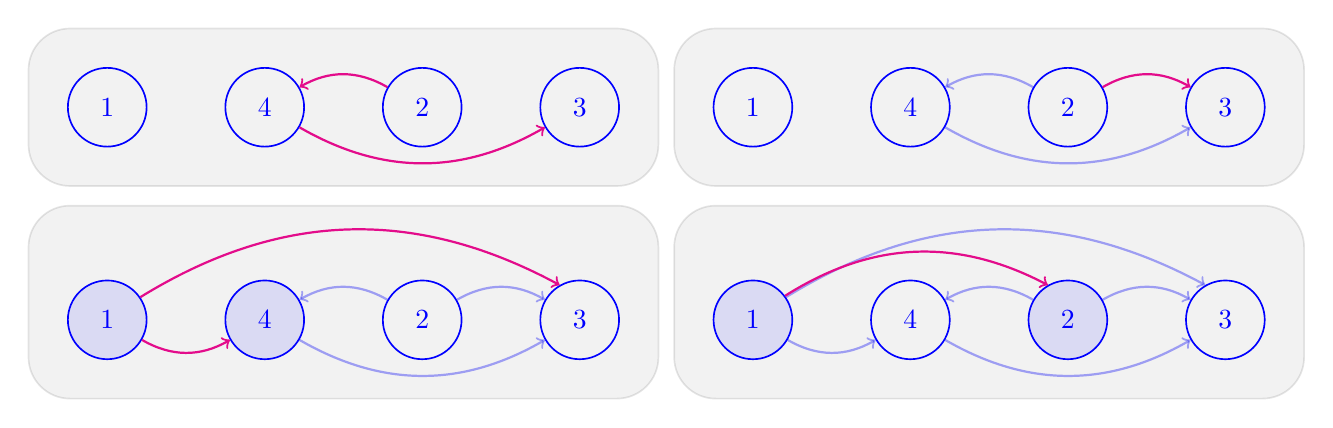
\begin{tikzpicture}[->, semithick]
		\tikzset{
		    tnode/.style= {circle, draw=blue, color=blue, minimum width=1cm},
		    tactive/.style= {circle, draw=blue, color=blue, fill=blue, fill opacity=0.1, text opacity=1, minimum width=1cm},
		    pold/.style= {above, black!5!blue, thick, opacity=.35},
		    pnew/.style= {below, black!5!magenta, thick},
		}
		
		\draw[fill=gray, opacity=0.1, rounded corners=15pt] (-1,1) rectangle (7,-1);
		\node[tnode] (s10) at (0, 0) {$1$};
		\node[tnode] (s40) at (2, 0) {$4$};
		\node[tnode] (s20) at (4, 0) {$2$};
		\node[tnode] (s30) at (6, 0) {$3$};
		
		\draw[fill=gray, opacity=0.1, rounded corners=15pt] (7.2,1) rectangle (15.2,-1);
		\node[tnode] (s11) at (8.2, 0) {$1$};
		\node[tnode] (s41) at (10.2, 0) {$4$};
		\node[tnode] (s21) at (12.2, 0) {$2$};
		\node[tnode] (s31) at (14.2, 0) {$3$};
		
		\draw[fill=gray, opacity=0.1, rounded corners=15pt] (-1,-1.25) rectangle (7,-3.7);
		\node[tactive] (s12) at (0, -2.7) {$1$};
		\node[tactive] (s42) at (2, -2.7) {$4$};
		\node[tnode] (s22) at (4, -2.7) {$2$};
		\node[tnode] (s32) at (6, -2.7) {$3$};
		
		\draw[fill=gray, opacity=0.1, rounded corners=15pt] (7.2,-1.25) rectangle (15.2,-3.7);
		\node[tactive] (s13) at (8.2, -2.7) {$1$};
		\node[tnode] (s43) at (10.2, -2.7) {$4$};
		\node[tactive] (s23) at (12.2, -2.7) {$2$};
		\node[tnode] (s33) at (14.2, -2.7) {$3$};
		
		\draw
		(s40) edge[pnew, bend right] (s30)
		(s20) edge[pnew, bend right] (s40)
		
		(s41) edge[pold, bend right] (s31)
		(s21) edge[pold, bend right] (s41)
		(s21) edge[pnew, bend left] (s31)
		
		(s42) edge[pold, bend right] (s32)
		(s22) edge[pold, bend right] (s42)
		(s22) edge[pold, bend left] (s32)
		(s12) edge[pnew, bend right] (s42)
		(s12) edge[pnew, bend left] (s32.120)
		
		(s43) edge[pold, bend right] (s33)
		(s23) edge[pold, bend right] (s43)
		(s23) edge[pold, bend left] (s33)
		(s13) edge[pold, bend right] (s43)
		(s13) edge[pold, bend left] (s33.120)
		(s13) edge[pnew, bend left] (s23.120);
	\end{tikzpicture}
	\captionof{figure}{Build steps for the $\sqsubset$ order on a trace $\tau = \pred{trace}{h, \emptyset, S, \mathds{P}}$ for some $h \in \mathsf{Storage}, S \in \mathsf{TState}$ and program $\mathds{P} = \left( \mathds{T}_1 ; \mathds{T}_4 \right) \| \left( \mathds{T}_2 ; \mathds{T}_3 \right)$. The purple edges are the ones created as part of the current step.}
	\label{fig:orderBuild}
\end{center}

\begin{defn}
	(\tpl\ Transactions order). Let $(N, E) = \pred{SG}{\tau}$ be the serialization graph in the definition of the \emph{transactions order} $\sqsubset$ for trace $\tau$:
	\begin{align*}
		\sqsubset_0 &= E^* \\
		\sqsubset_{n + 1} &=\ \sqsubset_n \cup \left( \sqsubset_n^\mathsf{id} ; \{ (i, j) \} ; \sqsubset_n^\mathsf{id} \right) \\
		&\text{where } i, j \in N \text{ and } i < j \\
		&\text{and } i \not\sqsubset_n j \text{ and } j \not\sqsubset_n i
	\end{align*}
\end{defn}

Now that we have a formal definition of the transactions order, we are required to show that $\sqsubset$ is a strict total order on the transactions appearing as part of a trace. We need it to be both strict and total, since we are interested in finding the effective serial execution order within a program run, therefore given two transactions, we must be able to find which one happened first. The strictness is required, since reflexivity of the order of transactions' execution does not make sense in this context. It follows that we can always find the minimal element of the relation, and once removed, a new one will be present. This particular property will prove very useful when proving the semantics equivalence.

\begin{thm}
	\label{thm:totOrder}
	(Order of transactions).
	The $\sqsubset$ relation is a strict total order on the set of transactions $N$ in $(N, E) = \pred{SG}{\tau}, \tau = \pred{trace}{h, \emptyset, \emptyset, \mathds{P}}, \mathds{P} \in \mathsf{Prog}, h \in \mathsf{Storage}$.

	\begin{proof}
	In order to show the theorem, we are required to prove that, for all $a, b, c \in N$:
	\begin{itemize}
		\item (Irreflexivity). $a \not\sqsubset a$
		\item (Asymmetry). If $a \sqsubset b$ then $b \not\sqsubset a$
		\item (Transitivity). If $a \sqsubset b$ and $b \sqsubset c$ then $a \sqsubset c$
		\item (Totality). $a \sqsubset b$ or $b \sqsubset a$ or $a = b$
	\end{itemize}
	
	Let's pick an arbitrary program $\mathds{P} \in \mathsf{Prog}$, initial storage $h \in \mathsf{Storage}$ and build its corresponding trace $\tau = \pred{trace}{h, \emptyset, \emptyset, \mathds{P}}$. We now consider the incrementally built $\sqsubset$ relation on $N$, where $(N, E) = \pred{SG}{\tau}$. \\
	\indline
	(Irreflexivity). The proof follows by induction on the number of $\sqsubset$ relation construction steps, $n$. Let's pick an arbitrary transaction identifier $a \in N$.
	
	{\parindent0pt
	\textit{Base case}: $n = 0$
	
	\textit{To show}: $a \not\sqsubset_0 a$
	
	By definition, we know that $\sqsubset_0 = E^*$, i.e. the transitive closure on the edges of the serialization graph $\pred{SG}{\tau}$. We directly obtain that $a \not\sqsubset_0 a$ from Theorem \ref{thm:sgAcyclic}, since $\pred{SG}{\tau}$ contains no cycles. \\
	
	\textit{Inductive case}: $n > 0$
	
	\textit{Inductive hypothesis}: $a \not\sqsubset_n a$
	
	\textit{To show}: $a \not\sqsubset_{n+1} a$
	
	Let's assume that $a \sqsubset_{n+1} a$ and, by definition, we know that it means that, for some $i, j \in N$ such that $i < j \land i \not\sqsubset_n j \land j \not\sqsubset_n i$ we have:
	\[
		(a, a) \in\ \sqsubset_n \cup \left( \sqsubset_n^\mathsf{id} ; \{ (i, j) \} ; \sqsubset_n ^\mathsf{id} \right)
	\]
	and by I.H. we can rewrite it as $(a, a) \in \left( \sqsubset_n^\mathsf{id} ; \{ (i, j) \} ; \sqsubset_n ^\mathsf{id} \right)$ given we assumed that $\sqsubset_n$ is irreflexive therefore $(a, a)$ cannot belong to it. It follows that it must be the case that $(a, i)$ and $(j, a)$ are in $\sqsubset_n^\mathsf{id}$ and moreover they must be in $\sqsubset_n$ given that $i < j$ and therefore $i \neq j$. By transitivity of $\sqsubset_n$, there must be a $(j, i) \in\ \sqsubset_n$. By contradiction we state that $a \not\sqsubset_{n+1} a$. \\
	}
	\indline
	(Asymmetry). The proof follows by induction on the number of $\sqsubset$ relation construction steps, $n$. Let's pick arbitrary transaction identifiers $a, b \in N$.
	
	{\parindent0pt
	\textit{Base case}: $n = 0$
	
	\textit{To show}: $a \sqsubset_0 b \implies b \not\sqsubset_0 a$
	
	By definition we know that $\sqsubset_0 = E^*$, i.e. the transitive closure on the edges of the serialization graph $\pred{SG}{\tau}$. Let's assume that $a \sqsubset_0 b$ meaning that $a \rightarrow^* b \in E$. We directly obtain that $b \not\sqsubset_0 a$ from Theorem \ref{thm:sgAcyclic}, as $\pred{SG}{\tau}$ contains no cycles. \\
	
	\textit{Inductive case}: $n > 0$
	
	\textit{Inductive hypothesis}: $a \sqsubset_n b \implies b \not\sqsubset_n a$
	
	\textit{To show}: $a \sqsubset_{n + 1} b \implies b \not\sqsubset_{n + 1} a$
	
	Let's assume that $a \sqsubset_{n + 1} b$ and by definition we know it means that, for some $i, j \in N$ such that $i < j \land i \not\sqsubset_n j \land j \not\sqsubset_n i$ we have:
	\[
		(a, b) \in\ \sqsubset_n \cup \left( \sqsubset_n^\mathsf{id} ; \{ (i, j) \} ; \sqsubset_n ^\mathsf{id} \right)
	\]
	\begin{itemize}
		\item If $a \sqsubset_n b$ we know by I.H. that $b \not\sqsubset_n a$. Let's instead assume that $(b, a) \in \left( \sqsubset_n^\mathsf{id} ; \{ (i, j) \} ; \sqsubset_n ^\mathsf{id} \right)$ from which it follows that there is a $(b, i) \in\ \sqsubset_n^\mathsf{id}$ and $(j, a) \in\ \sqsubset_n^\mathsf{id}$. By transitivity of $\sqsubset_n$ we obtain that $(j, i) \in\ \sqsubset_n^\mathsf{id}$ and moreover that $j \sqsubset_n i$ since $i \neq j$ as $i < j$ from our assumption. By contradiction we obtain that $(b, a) \not\in \left( \sqsubset_n^\mathsf{id} ; \{ (i, j) \} ; \sqsubset_n ^\mathsf{id} \right)$. We conclude that $b \not\sqsubset_{n + 1} a$.
		
		\item If $(a, b) \in \left( \sqsubset_n^\mathsf{id} ; \{ (i, j) \} ; \sqsubset_n ^\mathsf{id} \right)$ then this implies that there is a $(a, i) \in\ \sqsubset_n^\mathsf{id}$ and $(j, b) \in\ \sqsubset_n^\mathsf{id}$. Let's now assume that $(b, a) \in \left( \sqsubset_n^\mathsf{id} ; \{ (i, j) \} ; \sqsubset_n ^\mathsf{id} \right)$ meaning that there is a $(b, i) \in\ \sqsubset_n^\mathsf{id}$ and $(j, a) \in\ \sqsubset_n^\mathsf{id}$. By transitivity of $\sqsubset_n$ we obtain that $(j, i) \in\ \sqsubset_n^\mathsf{id}$ and moreover that $j \sqsubset_n i$ since $i \neq j$ as $i < j$. By contradiction we obtain that $(b, a) \not\in \left( \sqsubset_n^\mathsf{id} ; \{ (i, j) \} ; \sqsubset_n ^\mathsf{id} \right)$. We now assume that $b \sqsubset_n a$ which implies that $(b, a) \in\ \sqsubset_n^\mathsf{id}$. By transitivity of $\sqsubset_n$ we obtain that $(j, i) \in\ \sqsubset_n^\mathsf{id}$ and moreover that $j \sqsubset_n i$ since $i \neq j$ as $i < j$. By contradiction we obtain that $(b, a) \not\in\ \sqsubset_n$. We conclude that $b \not\sqsubset_{n + 1} a$.
	\end{itemize}
	}
	\ \\
	\indline
	(Transitivity). We are required to show that $\forall m \geq 1 \ldotp \sqsubset^m\ \subseteq\ \sqsubset$ The proof follows by induction on the number of self-composition steps, $m$.
	
	{\parindent0pt
	\textit{Base case}: $m = 1$
	
	\textit{To show}: $\sqsubset^1\ \subseteq\ \sqsubset$
	
	The result follows directly by definition $\sqsubset^1\ =\ \sqsubset\ \subseteq\ \sqsubset$. \\
	
	\textit{Inductive case}: $m > 1$
	
	\textit{Inductive hypothesis}: $\sqsubset^m\ \subseteq\ \sqsubset$
	
	\textit{To show}: $\sqsubset^{m + 1}\ \subseteq\ \sqsubset$
	\begin{align*}
		\sqsubset^{m + 1}
		&=\ \sqsubset^m ; \sqsubset \text{ by associativity} \\
		&\subseteq\ \sqsubset ; \sqsubset \text{ by I.H.} \\
		&\subseteq\ \sqsubset^2 \text{by definition} \\
		&\subseteq\ \sqsubset \text{ by Lemma \ref{lem:total2}}
	\end{align*}
	}
	
	(Totality). Let's pick arbitrary transaction identifiers $a, b \in N$ (\textsc{i}) for a finite $N$ and build the $\sqsubset$ relation on it until convergence, i.e. in a finite number of steps. If $(a, b) \in E^*$ or $(b, a) \in E^*$ then we know that either $a \sqsubset b$ or $b \sqsubset a$ holds. On the other hand if there is no edge connecting $a$ to $b$ or $b$ to $a$ in $E^*$ (\textsc{ii}) then:
	\begin{itemize}
		\item If $a = b$ then by irreflexivity of $\sqsubset$ we are done, as totality is met.
		\item Without loss of generality, we say that $a < b$ (\textsc{iii}). Given that the construction of $\sqsubset$ terminated in some $m > 0$ steps (being $N$ a finite set), by (\textsc{i}), (\textsc{ii}) and (\textsc{iii}) we know that there must exist a construction step $n$ such that $0 < n < m$ where the tuple $(a, b)$ was inserted in the relation given that $\sqsubset_{n-1} \cup \left( \sqsubset_{n-1}^\mathsf{id} ; \{(a,b)\} ; \sqsubset_{n-1}^\mathsf{id} \right) \implies a \sqsubset_n b \implies a \sqsubset b$. 
	\end{itemize}
	\end{proof}
\end{thm}
	
Theorem \ref{thm:totOrder} used the following lemma as the key component to prove the transitivity of the transactions order. Lemma \ref{lem:total2} shows that the relation composition of $\sqsubset$ with itself is included in $\sqsubset$.
	
\begin{lem}
	\label{lem:total2}
	Given a serialization graph $(N, E) = \pred{SG}{\tau}$ for $\tau = \pred{trace}{h, \emptyset, \emptyset, \mathds{P}}, \mathds{P} \in \mathsf{Prog}, h \in \mathsf{Storage}$, and the $\sqsubset$ relation on the set $N$ we say that $\sqsubset^2\ \subseteq\ \sqsubset$.
	
	{\parindent0pt
	\begin{proof}
	We proceed by induction on the number of $\sqsubset$ construction steps, $n$. \\
	\indline
	\textit{Base case}: $n = 0$
	
	\textit{To show}: $\sqsubset_0^2\ \subseteq\ \sqsubset_0$
	
	By definition we know that $\sqsubset_0 = E^*$, i.e. the transitive closure on the edges of the serialization graph $\pred{SG}{\tau}$. It follows that by definition of transitive closure, $\sqsubset_0^2\ = E^* ; E^* = E^*$ meaning that $\sqsubset_0^2\ \subseteq\ \sqsubset_0$. \\
	\indline
	\textit{Inductive case}: $n > 0$
	
	\textit{Inductive hypothesis}: $\sqsubset_n^2\ \subseteq\ \sqsubset_n$
	
	\textit{To show}: $\sqsubset_{n + 1}^2\ \subseteq\ \sqsubset_{n + 1}$
	
	We can rewrite the formula to be proven as the following, for some $i, j \in N$ such that $i < j \land i \not\sqsubset_n j \land j \not\sqsubset_n i$:
	\begin{align}
		\left( \sqsubset_n \cup \underbrace{\left( \sqsubset_n^\mathsf{id} ; \{ (i, j) \} ; \sqsubset_n^\mathsf{id} \right)}_{R} \right) ; \left( \sqsubset_n \cup \left( \sqsubset_n^\mathsf{id} ; \{ (i, j) \} ; \sqsubset_n^\mathsf{id} \right) \right) &\subseteq\ \sqsubset_{n + 1} \\
		\label{thm:total1}
		\underbrace{\sqsubset_n ; \sqsubset_n}_{\text{a}}
			\cup
		\underbrace{\sqsubset_n ; R}_{\text{b}}
			\cup
		\underbrace{R ; \sqsubset_n}_{\text{c}}
			\cup
		\underbrace{R ; R}_{\text{d}}
			&\subseteq\ \sqsubset_{n + 1} \text{ by distributivity}
	\end{align}
	It now suffices to show that each of the unioned sets in the l.h.s. of (\ref{thm:total1}) is a subset of $\sqsubset_{n + 1}$ itself. We start by proving that both sets $S =\ \sqsubset_n ; \sqsubset_n^\mathsf{id}$ and $S' =\ \sqsubset_n^\mathsf{id} ; \sqsubset_n$ are subsets of $\sqsubset_n^\mathsf{id}$ which will become useful in the following cases.
	\[
		\begin{array}{l @{\hspace{50pt}} l}
			\begin{aligned}
				S  &=\ \sqsubset_n ; \sqsubset_n^\mathsf{id} \\
					&=\ \sqsubset_n ; \left( \sqsubset_n \cup\ \pred{Id}{N} \right) \\
					&=\ \sqsubset_n ; \sqsubset_n \cup \sqsubset_n ; \pred{Id}{N} \\
					&=\ \sqsubset_n^2 \cup \sqsubset_n \\
					&\subseteq\ \sqsubset_n \cup \sqsubset_n \text{by I.H.} \\
					&\subseteq\ \sqsubset_n^\mathsf{id} \text{by definition}
				\end{aligned}
				&
				\begin{aligned}
					S' &=\ \sqsubset_n^\mathsf{id} ; \sqsubset_n \\
					&= \left( \sqsubset_n \cup\ \pred{Id}{N} \right) ; \sqsubset_n \\
					&=\ \sqsubset_n ; \sqsubset_n \cup\ \pred{Id}{N} ; \sqsubset_n \\
					&=\ \sqsubset_n^2 \cup \sqsubset_n \\
					&\subseteq\ \sqsubset_n \cup \sqsubset_n \text{ by I.H.} \\
					&\subseteq\ \sqsubset_n^\mathsf{id} \text{by definition}
				\end{aligned}
		\end{array}
	\]
	Next, we show that the set arising from the pre- and post-composition of the singleton relation $\{(i,j)\}$ with $\sqsubset_n^\mathsf{id}$, formally $S'' = \{ (i, j) \} ; \sqsubset_n^\mathsf{id} ; \{ (i, j) \}$ is always empty.
	\begin{align*}
		S'' = 
		\{ (i, j) \} ; \sqsubset_n^\mathsf{id} ; \{ (i, j) \}
			&=
		\{ (i, j) \} ; \left( \sqsubset_n \cup\ \pred{Id}{N} \right) ; \{ (i, j) \} \\
			&=
		\{ (i, j) \} ; \left( \sqsubset_n  ; \{ (i, j) \} \cup\ \pred{Id}{N}  ; \{ (i, j) \} \right) \\
			&=
		\{ (i, j) \} ; \left( \sqsubset_n ; \{ (i, j) \} \cup \{ (i, j) \} \right) \\
			&=
		\left( \{ (i, j) \} ; \sqsubset_n ; \{ (i, j) \} \right) \cup \left(\{ (i, j) \} ; \{ (i, j) \} \right) \\
		 	&=
		 \left( \{ (i, j) \} ; \sqsubset_n ; \{ (i, j) \} \right) = \emptyset
	\end{align*}
	The final fact is justified by the fact that we assumed that neither $(i, j)$ nor $(j, i)$ are part of the $\sqsubset_n$ relation, and the only way not to have a resulting empty set in this case, would be to have $j \sqsubset_n i$, which is clearly impossible.
	\begin{enumerate}[label=\alph*)]
		\item \textit{To show}: $\sqsubset_n ; \sqsubset_n\ \subseteq\ \sqsubset_{n + 1}$
			\begin{align*}
				\sqsubset_n ; \sqsubset_n\ &=\ \sqsubset_n^2 \\
				\text{by I.H.}&\subseteq\ \sqsubset_n\ \subseteq\ \sqsubset_{n + 1}
			\end{align*}
		\item \textit{To show}: $\sqsubset_n ; \left( \sqsubset_n^\mathsf{id} ; \{ (i, j) \} ; \sqsubset_n^\mathsf{id} \right) \subseteq\ \sqsubset_{n + 1}$
			\begin{align*}
				\sqsubset_n ; \left( \sqsubset_n^\mathsf{id} ; \{ (i, j) \} ; \sqsubset_n^\mathsf{id} \right) &= \left( \sqsubset_n ; \sqsubset_n^\mathsf{id} ; \{ (i, j) \} \right) ; \sqsubset_n^\mathsf{id} \text{ by associativity} \\
				&= \left( S ; \{ (i, j) \} \right) ; \sqsubset_n^\mathsf{id} \text{ by associativity} \\
				&\subseteq\ \sqsubset_n^\mathsf{id} ; \{ (i, j) \} ; \sqsubset_n^\mathsf{id} \\
				&\subseteq\ \sqsubset_{n + 1}
			\end{align*}
		\item \textit{To show}: $\left( \sqsubset_n^\mathsf{id} ; \{ (i, j) \} ; \sqsubset_n^\mathsf{id} \right) ; \sqsubset_n \subseteq\ \sqsubset_{n + 1}$
			\begin{align*}
				\left( \sqsubset_n^\mathsf{id} ; \{ (i, j) \} ; \sqsubset_n^\mathsf{id} \right) ; \sqsubset_n &=\ \sqsubset_n^\mathsf{id} ; \left( \{ (i, j) \} ; \sqsubset_n^\mathsf{id} ; \sqsubset_n \right) \text{ by associativity} \\
				&=\ \sqsubset_n^\mathsf{id} ; \left( \{ (i, j) \} ; S' \right) \text{ by associativity} \\
				&\subseteq\ \sqsubset_n^\mathsf{id} ; \{ (i, j) \} ; \sqsubset_n^\mathsf{id} \\
				&\subseteq\ \sqsubset_{n + 1}
			\end{align*}
		\item \textit{To show}: $\left( \sqsubset_n^\mathsf{id} ; \{ (i, j) \} ; \sqsubset_n^\mathsf{id} \right) ; \left( \sqsubset_n^\mathsf{id} ; \{ (i, j) \} ; \sqsubset_n^\mathsf{id} \right) \subseteq\ \sqsubset_{n + 1}$
			\iffalse
			Let's assume that $\left( \sqsubset_n^\mathsf{id} ; \{ (i, j) \} ; \sqsubset_n^\mathsf{id} \right) ; \left( \sqsubset_n^\mathsf{id} ; \{ (i, j) \} ; \sqsubset_n^\mathsf{id} \right) \neq \emptyset$ meaning that the set at least contains a tuple $(a, b)$, for $a, b \in N$. 
			\begin{align}
				(a, b) \in \left( \sqsubset_n^\mathsf{id} ; \{ (i, j) \} ; \sqsubset_n^\mathsf{id} \right) ; \left( \sqsubset_n^\mathsf{id} ; \{ (i, j) \} ; \sqsubset_n^\mathsf{id} \right)
					&\iff \\
				\exists c \ldotp (a, c) \in \left( \sqsubset_n^\mathsf{id} ; \{ (i, j) \} ; \sqsubset_n^\mathsf{id} \right) \land (c, b) \in \left( \sqsubset_n^\mathsf{id} ; \{ (i, j) \} ; \sqsubset_n^\mathsf{id} \right)
					&\iff \\
				\exists c \ldotp (a, i) \in\ \sqsubset_n^\mathsf{id} \land (i, j) \in  \{(i, j)\} \land (j, c) \in\ \sqsubset_n^\mathsf{id} \\ \land (c, i) \in\ \sqsubset_n^\mathsf{id} \land (i, j) \in  \{(i, j)\} \land (j, b) \in\ \sqsubset_n^\mathsf{id}
					&\implies \\
				\label{thm:total4} \exists c \ldotp (j, c) \in\ \sqsubset_n^\mathsf{id} \land (c, i) \in\ \sqsubset_n^\mathsf{id}
			\end{align}
			We know that $i \neq j$ since $i < j$ so the proof proceeds with a case-by-case analysis on $c$.
			\begin{itemize}
				\item If $c = i$ then we know that $c \neq j$ and by (\ref{thm:total4}) we have that $(j, i) \in\ \sqsubset_n^\mathsf{id} \land (i, i) \in\ \sqsubset_n^\mathsf{id}$ from which it follows that $(j, i) \in\ \sqsubset_n$, a contradiction.
				\item If $c = j$ then we know that $c \neq i$ and by (\ref{thm:total4}) we have that $(j, j) \in\ \sqsubset_n^\mathsf{id} \land (j, i) \in\ \sqsubset_n^\mathsf{id}$ from which it follows that $(j, i) \in\ \sqsubset_n$, a contradiction.
				\item If $c \neq i$ and $c \neq j$ then (\ref{thm:total4}) it follows that $(j, c) \in\ \sqsubset_n \land (c, i) \in\ \sqsubset_n$. By I.H. we know that $\sqsubset_n^2\ \subseteq\ \sqsubset_n$. By definition we know that if $(j, c) \in\ \sqsubset_n$ and $(c, i) \in\ \sqsubset_n$ then $(j, i) \in\ \sqsubset_n^2$. By I.H. this means that $(j, i) \in\ \sqsubset_n$ which is again a contradiction.
			\end{itemize}
			By contradiction we conclude that $\left( \sqsubset_n^\mathsf{id} ; \{ (i, j) \} ; \sqsubset_n^\mathsf{id} \right) ; \left( \sqsubset_n^\mathsf{id} ; \{ (i, j) \} ; \sqsubset_n^\mathsf{id} \right) = \emptyset$ meaning that $\left( \sqsubset_n^\mathsf{id} ; \{ (i, j) \} ; \sqsubset_n^\mathsf{id} \right) ; \left( \sqsubset_n^\mathsf{id} ; \{ (i, j) \} ; \sqsubset_n^\mathsf{id} \right) \subseteq\ \sqsubset_{n + 1}$.
			
			Direct proof.
			\fi
			\begin{align*}
				\left( \sqsubset_n^\mathsf{id} ; \{ (i, j) \} ; \sqsubset_n^\mathsf{id} \right) ; \left( \sqsubset_n^\mathsf{id} ; \{ (i, j) \} ; \sqsubset_n^\mathsf{id} \right)
					&=
				\left( \sqsubset_n^\mathsf{id} ; \{ (i, j) \} \right) ; \left( \sqsubset_n^\mathsf{id} ; \left( \sqsubset_n^\mathsf{id} ; \{ (i, j) \} ; \sqsubset_n^\mathsf{id} \right) \right) \\
					&=
				\left( \sqsubset_n^\mathsf{id} ; \{ (i, j) \} \right) ; \left( \left( \sqsubset_n^\mathsf{id} ;  \sqsubset_n^\mathsf{id} \right) ; \left( \{ (i, j) \} ; \sqsubset_n^\mathsf{id} \right) \right) \\
					&=
				\left( \sqsubset_n^\mathsf{id} ; \{ (i, j) \} \right) ; \left( \sqsubset_n^\mathsf{id} ; \left( \{ (i, j) \} ; \sqsubset_n^\mathsf{id} \right) \right) \\
					&=\
				\sqsubset_n^\mathsf{id} ; \left( \{ (i, j) \} ; \sqsubset_n^\mathsf{id} ; \{ (i, j) \} \right) ; \sqsubset_n^\mathsf{id} \\
					&=\
				\sqsubset_n^\mathsf{id} ; \emptyset ; \sqsubset_n^\mathsf{id} \\
					&= \emptyset \subseteq\ \sqsubset_{n+1}
			\end{align*}
	\end{enumerate}
	\end{proof}
	}
\end{lem}